\documentclass[parskip=full]{scrartcl}
\usepackage[utf8]{inputenc} % use utf8 file encoding for TeX sources
\usepackage[T1]{fontenc}    % avoid garbled Unicode text in pdf
\usepackage[german]{babel}  % german hyphenation, quotes, etc
\usepackage{hyperref}       % detailed hyperlink/pdf configuration
\hypersetup{                % ‘texdoc hyperref‘ for options
pdftitle={SWT1: Lastenheftvorlage},%
bookmarks=true,%
}
\usepackage{graphicx}       % provides commands for including figures
\usepackage{csquotes}       % provides \enquote{} macro for "quotes"
\usepackage[nonumberlist]{glossaries}     % provides glossary commands
\usepackage{enumitem}

\makenoidxglossaries
%
% % Glossareinträge
%
% % TODO Glossar bearbeiten
%
\newglossaryentry{iMage}
{
	name=iMage,
	description={Bildbearbeitungsprogramm der Firma \gls{Pear Corp.}.},
}
\newglossaryentry{Pear Corp.}
{
	name=Pear Corp.,
	description={Auftraggeber für das Produkt und Besitzer des Produktes \gls{iMage}.}
}
\newglossaryentry{Kunstfilter}
{
	name=Kunstfilter,
	description={Computeralgorithmus, welcher Bilder mit bestimmten Methoden nachstellt.}
}
\newglossaryentry{Java}
{
	name=Java,
	description={Programmiersprache. Java Runtime Environment (JRE) ist ein Teil der Sprache und kann seperat heruntergeladen werden. JRE wird für das Ausführen der Datei benötigt.}
}
\newglossaryentry{Geometrify}
{
	name=Geometrify,
	description={Ein \gls{Kunstfilter}, der Bilder mit geometrischen Primitven (Dreiecke, Vierecke) nachstellt. Geometrify ist im Produkt standardmäßig mit enthalten.}
}
\newglossaryentry{Schnittstelle}
{
	name=Schnittstelle,
	plural=Schnittstellen,
	description={Eine Art "offener Code". Durche eine Schnittstelle können externe Programme (\glspl{Plug-In}) ohne viel Aufwand in das Programm mit der Schnittstelle integriert werden.}
}
\newglossaryentry{Plug-In}
{
	name=Plug.In,
	plural=Plug-Ins,
	description={Bausteinartiger Code-Schnipsel. Plug-Ins können durch \glspl{Schnittstelle} in Programme integriert werden.}
}
\newglossaryentry{In-App-Kauf}
{
	name=In-App-Kauf,
	description={Kauf in einem \gls{In-App Store}.},
	plural=In-App-Käufe,
}
\newglossaryentry{Kunde}
{
	name=Kunde,
	plural=Kunden,
	description={Benutzer des Produktes \gls{iMage}.}
}
\newglossaryentry{Bank}
{
	name=Bank,
	plural=Banken,
	description={Kreditinstitut. Ein \gls{Kunde} besitzt ein Konto bei einer Bank, um \glspl{In-App-Kauf} zu tätigen.}
}
\newglossaryentry{Entwickler}
{
	name=Entwickler,
	description={Entwickelt das Produkt \gls{iMage} und verschiedene \gls{Kunstfilter}, die im \gls{In-App Store} angeboten werden.}
}
\newglossaryentry{In-App Store}
{
	name=In-App Store,
	plural=In-App Stores,
	description={Eine Funktion von \gls{iMage}. Über dem In-App Store kann ein \gls{Kunde} Käufe von \gls{Kunstfilter} tätigen.}
}
\newglossaryentry{Betriebssystem}
{
	name=Betriebssystem,
	plural=Betriebssysteme,
	description={Software, die es ermöglicht, andere Programme einfach auszuführen. Beispiele sind: Microsoft Windows, Apple MacOS, Ubuntu, Linux Mint.}
}

\title{SWT1: Lastenheftvorlage}
\author{Joshua Eilebrecht, 1939691}

\begin{document}

\maketitle

%
% % Hier beginnt die Gliederung des Lastenhefts
%
% % TODO Glossareinträge einfügen
%
\section{Zielbestimmung}
Das Produkt \gls{iMage} von \gls{Pear Corp.} soll durch das Produkt in der Lage sein, \gls{Kunstfilter} ohne großen Aufwand mit sich selbst zu integrieren.

\section{Produkteinsatz}
Das Produkt dient zur Verwaltung der in iMage integrierten Kunstfilter.

Zielgruppe: Benutzer des Produktes iMage.

Plattform:PC mit einem \gls{Java}-unterstützenden \gls{Betriebssystem}.

\section{Funktionale Anforderungen}
\begin{itemize}[nosep]
\item[FA10] Einfügen und Entfernen von Kunstfilter.
\item[FA20] Vollkommene Unterstützung der zugefügten Kunstfiltern.
\item[FA30] Mitlieferung des Kunstfilters \gls{Geometrify}.
\item[FA40] Sofortige Bereitstellung der zugefügten Kunstfilter.
\item[FA50] Problemlose Ausführung der Kunstfilter durch iMage.
\end{itemize}

\newpage
\section{Produktdaten}
\begin{itemize}[nosep]
\item[PD10] Es sind bestimmte Verzeichnisse für das Erkennen und Integrieren von Kunstfilter bei Änderung einzulesen.
\item[PD20] Falls ein Kunstfilter entfernt werden, ist das Entfernen der mit dem Filter verknüpfte Dateien zu löschen.
\item[PD30] Es ist der Zugriff auf iMage erforderlich.
\end{itemize}

\section{Nichtfunktionale Anforderungen}
\begin{itemize}[nosep]
\item[NF10] Alle Kunstfilter müssen mit der selben \gls{Schnittstelle} funktionieren können.
\item[NF20] Falls beim Verarbeiten eines Bildes entstehen, muss der Kunstfilter selbst das Problem behandelt werden oder an iMage weitergereicht werden.
\item[ND30] Die Filter müssen unabhängig voneinander funktionieren können.
\end{itemize}

\section{Systemmodelle}

\subsection{Szenarien}
\subsubsection{Image als Kunstfilterapp}
%
% % TODO weiter verbessern
%
Die Firma Pear Corp. möchte das Produkt iMage als Kunstfilter-App vertreiben. Hierfür soll auf eine erweiterbare \glspl{Plug-In} Architektur gesetzt werden, welche es ermöglicht, einzelne Kunstfilter als Plug-Ins zu modellieren. In der Basis-Variante soll hierbei zunächst ein Kunstfilter zur Abstraktion eines Bilds durch geometrische Primitive (Dreiecke, Vierecke, …) ausgeliefert werden. Weitere Filter sollen per \glspl{In-App-Kauf} erworben werden können. Nach dem Kauf wird der Filter in die entsprechende Position geladen und in iMage integriert. Bereits gekaufte Filter können jeder Zeit weiter heruntergeladen werden.
Der Kunstfilter der Basis-Variante mit Namen Geometrify soll in der Lage sein, ein gegebenes Bild durch Hinzufügen vieler gleichartiger Primitive nachzubilden. Hierbei soll das verwendete Primitiv gewählt werden können.
Die Auswahl soll per Auswahlmenü in der graphischen Benutzeroberfläche von iMage ermöglicht werden. Nach der Auswahl des Primitivs soll eine Vorschau des Filtereffektes für das aktuelle Bild angezeigt werden. Die Berechnung des Vorschaubilds soll in Echtzeit möglich sein. Hierzu soll beim Laden des Bilds durch den Nutzer zusätzlich eine Variante mit niedriger Auflösung abgespeichert werden. Nach der Beendigung der App sollen diese Bilder zur Verbesserung der App an die Pear-Corp.-Firmenzentrale übermittelt werden.
Kunstfilter können jederzeit vom Benutzer installiert oder deinstalliert werden.
\subsection{Anwendungsfälle}
\subsubsection{Kauf und Benutzung eines Kunstfilters}
\begin{center}
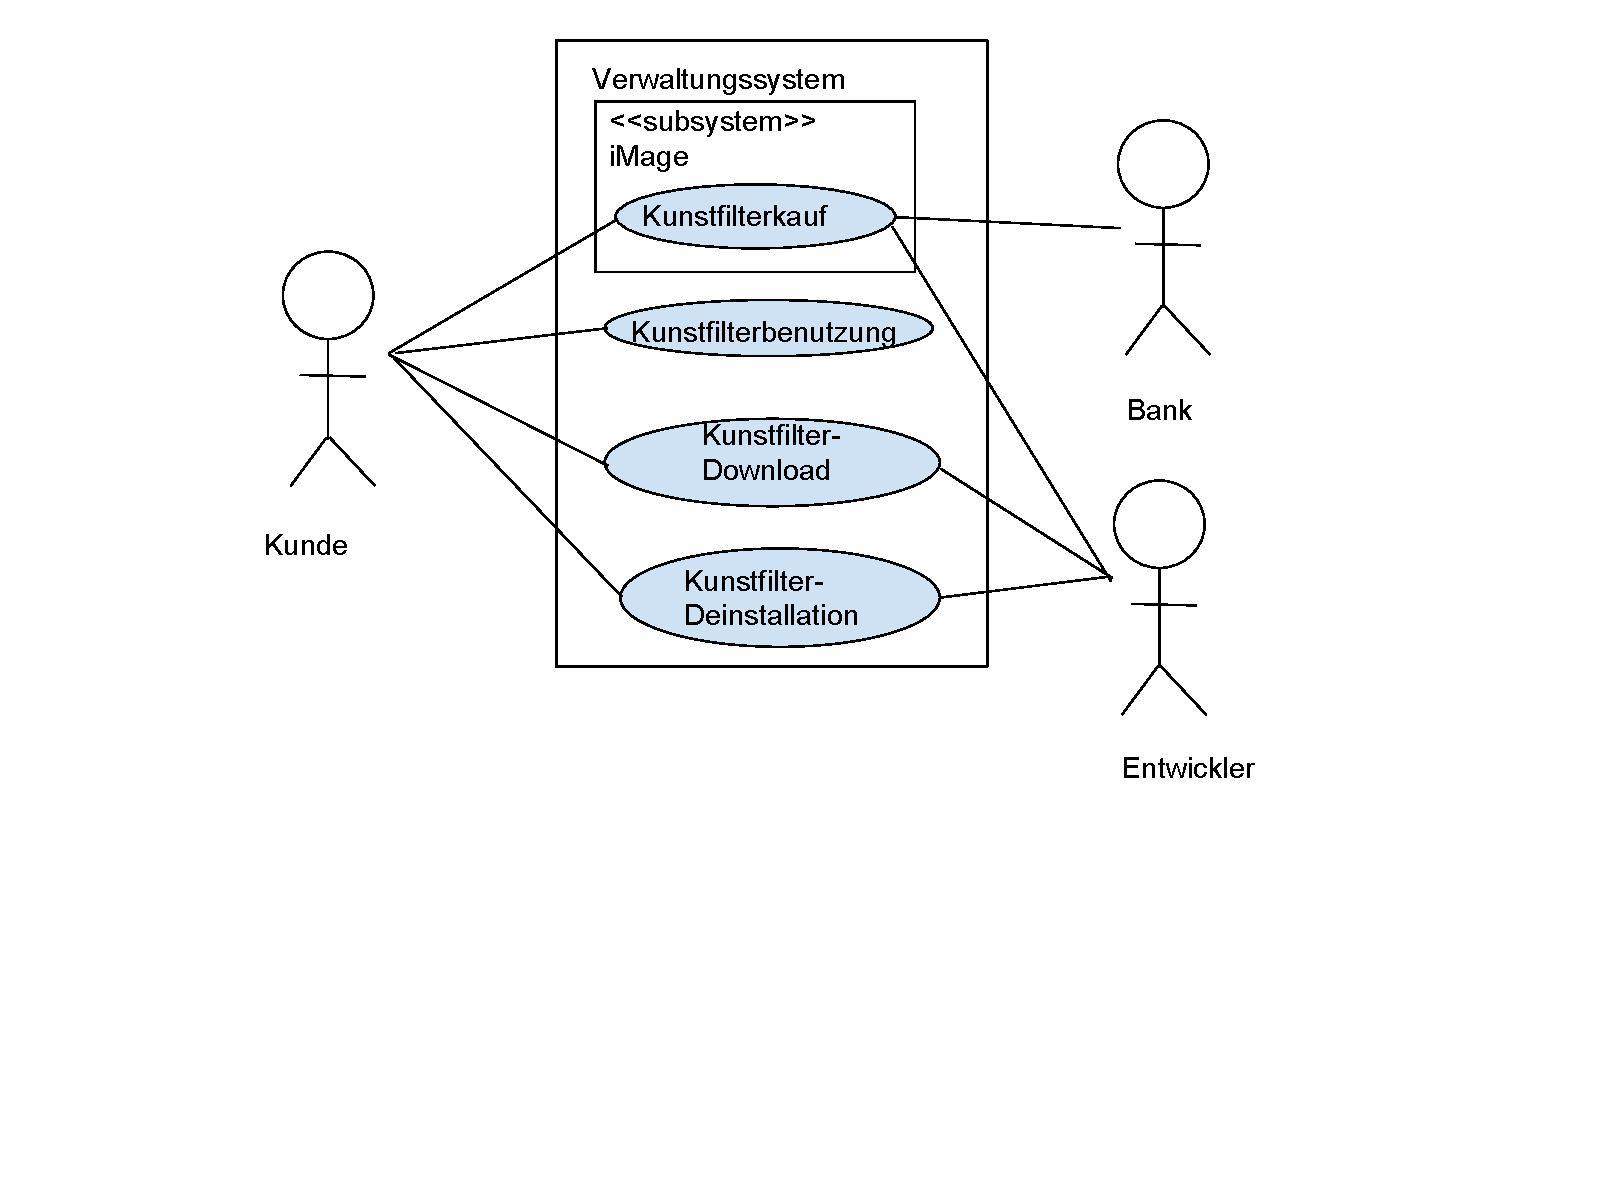
\includegraphics[width=0.8\textwidth]{szenario_iMage_als_Kunstfilterapp.pdf}
\end{center}

Akteure: \gls{Kunde}, \gls{Bank}, \gls{Entwickler}.

Anwendungsfälle: Kunstfilterkauf, Kunstfilterdownload, Kunstfilterbenutzung, Kunstfilterdeinstallation.

Textuelle Beschreibung:
Der Entwickler entwickelt einen Kunstfilter und stellt diesen im \gls{In-App Store} von iMage zu Verfügung. Der Kunde kauft diesen Kunstfilter über iMage. Die Bank verifiziert den vom Kunden getätigten Kauf.
Der Entwickler stellt den gekauften Kunstfilter als Download bereit. Der Kunde lädt sich diesen nach dem Kauf herunter.
Der Kunde benutzt den gekauften Filter. Der Filter generiert Bilder mit niedriger Auflösung und der Entwickler greift auf diese Bilder zu, um den Filter zu verbessern.
Der Kunde deinstalliert nach Bedarf den Filter.


%
% % Automatisch generiertes Glossar (Latex zwei mal ausführen um Glossar anzuzeigen)
%
%\glsaddall % das sorgt dafür, dass alles Glossareinträge gedruckt werden, nicht nur die verwendeten. Das sollte nicht nötig sein!

\printnoidxglossaries




\end{document}
